
\documentclass[tikz,border=7pt]{standalone}
\usepackage[utf8]{inputenc}
\usepackage[T1]{fontenc}
\usepackage{amsmath}
\usepackage{xcolor}
\usetikzlibrary{arrows.meta,calc,angles,quotes,patterns,positioning}
\definecolor{brand}{HTML}{1E3A8A}
\definecolor{brandtwo}{HTML}{2563EB}
\definecolor{accentred}{HTML}{EF4444}
\definecolor{accentgreen}{HTML}{16A34A}
\definecolor{accentorange}{HTML}{F59E0B}
\definecolor{muted}{HTML}{64748B}
\definecolor{lightblue}{HTML}{EEF6FF}
\tikzset{force/.style={-{Latex[length=3mm]}, line width=1.15pt}, axis/.style={-{Latex[length=2mm]}, line width=.8pt, color=muted}, body/.style={draw=brandtwo, fill=lightblue, line width=1pt, rounded corners=2pt}, lab/.style={font=\small, text=brand}, sml/.style={font=\scriptsize, text=muted}}
\begin{document}

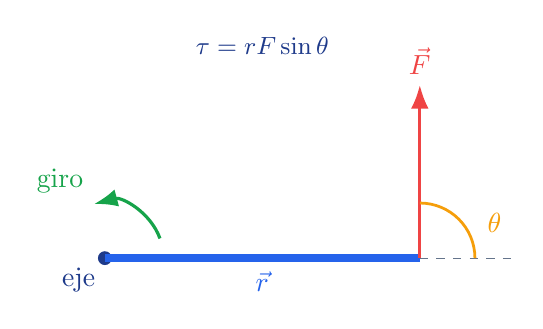
\begin{tikzpicture}[scale=1]
\fill[brand] (0,0) circle (2.5pt) node[below left] {eje};
\draw[line width=3pt, color=brandtwo] (0,0)--(4,0) node[midway,below] {$\vec r$};
\draw[force,color=accentred] (4,0)--++(0,2.2) node[above] {$\vec F$};
\draw[dashed,muted] (4,0)--++(1.2,0); \draw[accentorange,line width=1pt] (4.7,0) arc[start angle=0,end angle=90,radius=.7]; \node[text=accentorange] at (4.95,.45) {$\theta$};
\draw[force,color=accentgreen] (.7,.25) arc[start angle=20,end angle=105,radius=.7] node[above left] {giro};
\node[lab] at (2,2.7) {$\tau=rF\sin\theta$};
\end{tikzpicture}

\end{document}